\documentclass{bioinfo}
\copyrightyear{2005}
\pubyear{2005}

\usepackage[hyphens]{url}

\begin{document}
\firstpage{1}


\newcommand{\OnePhaseone}{Phase1\_Chr1}
\newcommand{\NinteenPhaseone}{Phase1\_Chr19}
\newcommand{\SevenPhaseone}{Phase1\_Chr1-7}
\newcommand{\OnePhasethree}{Phase3\_Chr1}
\newcommand{\ThreePhasethree}{Phase3\_Chr1-3}
\newcommand{\FullPhasethree}{Phase3\_Chr1-22}

\title[MapReduce Clustering]{Scalable Clustering of Genotype Information using MapReduce}
\author[O'Brien \textit{et~al}]{Aidan R O'Brien\,$^{1}$, Fabian A Buske\,$^{2}$ and Denis C. Bauer\,$^1$\footnote{to whom correspondence should be addressed}}
\address{$^{1}$CSIRO, Digital Productivity Flagship, 11 Julius Av, 2113, Sydney, Australia\\
$^{2}$Cancer Epigenetics Program, Cancer Research Division, Kinghorn Cancer Centre, Garvan Institute of Medical Research, 384 Victoria St, 2010, Sydney, Australia}

\history{Received on XXXXX; revised on XXXXX; accepted on XXXXX}

\editor{Associate Editor: XXXXXXX}

\maketitle

\begin{abstract}

\section{Motivation:}
Processing genomic information from whole genome sequence studies pose computational challenges due to the unprecedented data volume generated, which render transitional approaches insufficient. However, by utilising advancements in modern hardware accelerators and data processing we can provide the means for scalable solutions. We therefore aim to provide the interface between standard genomic data formats and advanced and scalable analysis libraries like Mahout. 
\section{Results:}
We achieve an 2-fold speedup by using the scalable k-means MapReduce implementation over the equivalent analysis performed in R, by comparable accuracy. However, the real benefit lies in scaling beyond R's capability to a population-size analysis. We successfully clustered more than 2,500 individuals each having more than 19 Million variants. 

\section{Availability:}
Using modern compute paradigms is essential to scale to modern genomic research in an efficient sustainable way. 

\section{Contact:} \href{Denis.Bauer@CSIRO.au}{Denis.Bauer@CSIRO.au}
\end{abstract}

\section{Introduction}

Grouping individuals based on the genomic profile is a commonly performed tasks to identify population structure~\cite{Gao2007} or elucidate different haplotype involvement in diseases susceptibility~\cite{Laitman2013}.  Traditionally both the number of individuals and included genotypes, typically from SNP arrays, were relatively small and libraries in Bioconductor sufficient. However, recent technological advances in whole genome sequencing have made population-scale sequencing feasible. It is hence economical to generate studies with sample sizes currently reserved for larger consortia such as the 1000 genomes project~\cite{1KG2012} or the cancer genome atlas (TCGA)~\cite{TCGA2013}. At the same time, whole genome sequencing enables the inclusion of rare or even somatic mutations in the analysis, increasing the feature space by orders of magnitude. This drastic increase in both sample numbers and features per sample requires a massively parallel approach to data processing. 

As a result of these big data challenges, MapReduce approaches are increasingly being used in bioinformatics (for reviews see~\cite{Zou2013, Qiu2010,Taylor2010}). This is especially the case for sequence analysis tasks, such as read mapping~\cite{Schatz2009}, duplicate removal~\cite{Jourdren2012}, and variant calling~\cite{Langmead2009, McKenna2010} as well as Genome Wide Analysis Study based tasks~\cite{Huang2013, Guo2014}.

%Mention Goolge's population clustering in the intro

At the same time, theoretical computer scientists adapt MapReduce paradigms to cope with the iterative nature of machine learning tasks~\cite{Chu2009}. Specifically, the Mahout project \url{https://mahout.apache.org/} has been developed extensively~\cite{Ranger2007, Owen2011} and was successfully applied in the clinical informatics space~\cite{Dong2013}.

In this paper we link the two areas of parallel machine learning and bioinformatics by providing an interface between Mahout and the standard variant data format, variant call format (VCF)~\cite{1KG2012}, which opens up the application of Mahout's different machine learning algorithms to be applied to genotype-based tasks. 

To demonstrate the capability we cluster variant datasets from the 1000 genomes project to determine population structure using the k-means clustering algorithm available in Mahout. In the first section we benchmark the performance and accuracy of Mahout's implementations against a standard R based implementation on a reduced version of the data and in the last two sections we investigate how Mahout scales to either more samples or more features per samples.   

%SeqWare~{OConnor2010} Libraries \cite{Doering2008,Schumacher2014,Nordberg2013}


\section*{Results and discussion}


% COMPARISON TO R
\subsection*{Clustering in Mahout uses less memory than in R}
In this section, we compare the runtime between the k-means clustering implementation in R and Mahout for the small \NinteenPhaseone\ dataset (see Methods). 
We measured the runtime separately for pre-processing stage as well as the clustering stage. 
With Hadoop, pre-processing the data takes approximately 3 minutes, with an allocation of up to 2GB memory per container. The resulting data is stored as a Hadoop 'SequenceFile' of about 835MB in size.
Conversely,  pre-processing the data to R's in-memory matrix takes 56 minutes and uses 17.7GB memory. 
K-means clustering the data, however, is faster with R, using 7s, whereas Mahout takes just over 9 minutes. See Table~\ref{datasetsTime}. \\
Due to the relatively small number of variants, cluster performance is very poor for both methods, with the best Adjusted Rand Index score for clustering individuals in one of 4 populations (see Methods) being 0.730 in Mahout and 0.614 in R (see Table~\ref{datasetsAcc}).

Although the overall Mahout pipeline is about 43 minutes faster than R's, Mahout's k-means clustering takes two orders of magnitude longer. 
This is likely due to the additional overhead involved in spawning the map and reduce processes, and distributing the data between nodes.
R, on the other hand, already has the entire matrix in-memory, on a single machine, this speeds up the clustering significantly as no disk-access or networking is required. However, the amount of memory available on a single machine can quickly becomes a limiting factor. As an example, the entire set of 1000 Genome Project Phase 3 variants would require approximately 1.6TB to be completely loaded into memory as a double-precision matrix (see Table~\ref{datasetsAcc}). 

Also, although Hadoop, in this case, has access to a total of 36GB of memory distributed over 3 machines, the container size is only 2GB. Therefore, we could
easily run the same job on a single 12GB node, at the expense of time. 

This example demonstrates the potential for scalability in Hadoop, compared to single machine solutions, in respect to it's potential applications to genomics. We will proceed to demonstrate that Mahout can expand with relative ease to encompass larger data, although this depends on the task and how it can be parallelized.


% SCALING UP FEATURES IN MAHOUT
\subsection*{Hadoop scales to 19 Million genomic variants}
In this section we demonstrate Mahout's scaling ability by increasing the numbers of features (variants per sample).



R therefore was not able to perform the clustering on even the second smallest dataset (\OnePhaseone , 3 Million variants). This dataset, stored as a double-precision matrix would consume approximately 26GB memory, hence why the in-memory implementation of R fails. Therefore we will only
report the results for Hadoop.
On this dataset Hadoop's pre-processing takes 7 minutes, using the same container size as the smaller dataset. Clustering takes 23 minutes.
The clustering accuracy increased by 35\% to 0.891, compared to the performance on \NinteenPhaseone\ (see Table~\ref{datasetsAcc}).

To perform k-means clustering on the entire dataset in a reasonable amount of time would require a larger cluster with more memory per container.
This is because each Map task loads the entire feature vector for the clusters into memory.
Although we could increase the container size to the full 12GB per node, this would mean only 3 containers (1 per node) could run simultaneously, rather than the maximum of 18, and would greatly increase the processing time.
Pre-processing the data, however, does scale to the entire feature-set, without an increase in container memory. Having the data in the distributed
SequenceFile format opens the door to other distributed analysis techniques.

While R does not scale to either of the two orders of magnitude incased datasets, We have demonstrated Hadoop to cope well with up to 70 Million variants. Although k-means clustering with a feature-set of this size is not feasible on a compute cluster of this size, clustering a smaller subset of the genome is a trivial task.

% SCALING UP SAMPLES IN MAHOUT
\subsection*{Hadoop scales effortless to an order of magnitude more samples}
In this section we investigate Mahout's ability to scale with more samples, i.e. the 1092 individuals in the Phase 1 dataset and the 2535 individuals in the Phase 3 dataset.
We used the \SevenPhaseone\ and the \ThreePhasethree\ data-sets specifically because they both contain a similar number of variants (19 million).
The container size required for pre-processing the data is identical for both datasets, with the Phase 3 dataset requiring less than double the time of the smaller Phase 1 dataset.
In this case, due to the number of Feature Vectors increasing, rather than the feature size, the memory requirements for k-means clustering should remain similar, as the cluster centres loaded into the containers' memory are approximately the same size.
This proved to be the case, as 4GB allocated per container was the minimum for both datasets. The time to complete clustering was much higher though,
especially due to the fact that only 9 4GB containers can run simultaneously, rather than the 24 1.5GB containers. 
The clustering accuracy is 0.816 for the Phase 1 dataset and 0.xxx for the Phase 3 dataset.

%TODO: can you think of a less general statement as conclusion
Scaling effortless to massively more samples is the strength of Hadoop, hence compute problems need to be carefully designed to harness this ability.  


\section*{Conclusion}
In this paper we have applied Mahout's k-means clustering to the task of genotype based population. 
We provide an interface from VCF format to Hadoop and Mahout, and a toolset to interpret Mahout's clustering output (see Figure 1)
We find that on small datasets the actual clustering stage is two orders of magnitudes slower in Mahout compared to R (9 minutes vs 7 seconds), likely due to the overhead of setting up and co-ordinating the communication between the Hadoop nodes. 
However, increasing either the number of samples or the number of features per sample quickly exceeds the ability of R.
Mahout on the other hand scales effortlessly to more than twice the number samples (2,535) and can process data with over 79 Million features per samples.
As the memory required for k-means clustering directly scales with the number of features per sample, we observe that Mahout's implementation
of k-means does not scale to the entire exome dataset, unless memory per container were increased beyond the limits of our cluster.
However, this might be resolved once Mahout moves from MapReduce to a domain-specific language for linear algebraic operations on top of Apache Spark \url{http://spark.apache.org/}.

In conclusion, Mahout offers a scalable out-of-the box solution that is directly applicable to genotype-based clustering for population or family association. 

%This efficient a high performance in-memory map-reduce system has already demonstrated to deliver a  50x speed-up on a whole-genome dataset compared to usual multithreaded approaches, see ADAM~\cite{Massie2013}


\begin{methods}
\section{Methods}
\subsection*{Datasets}
We used variant call format (VCF) files from phase 1 and 3 of the 1000 Genomes Project.
The VCF files contain information about the genetic variants between each of the 1092 and 2,535 individuals respectively and a reference genome derived from GRCh37. 
Each of the VCF files contain the variants in one chromosome, and we only use the 22 autosomes.
Metadata available from the 1000 Genomes Consortium specifies additional attributes for each individual, including population and familial data.\\
We used different subsets of the data for different comparisons. For example, to be able to compare Hadoop with R, we used a subset of the entire human variant dataset containing only chromosome 19 variants (\NinteenPhaseone ).
Scaling up using Hadoop, we investigate how the accuracy improves when using more variants from the genome with \SevenPhaseone\ and \FullPhasethree, which include chromosome 1-7 and the full genome, respectively.
Table~\ref{datasets} contains an overview of the datasets.

\subsection*{Hardware and Software}
We processed the data using a cluster of five VMs on the Microsoft Azure cloud service. Three of the VMs, the 'worker nodes', each have 14GB memory and and 8 CPU cores. These three VMs run the Hadoop2 NodeManager. The NodeManager manages the Yet Another Resource Negotiator (YARN) 'containers', where YARN allows the user
to specify the resources allocated to each container.
The fourth VM runs the HDFS NameNode, ResourceManager and monitoring services, and the fifth VM, a small, single core machine, runs the Cloudera manager service.
With this hardware setup, we can run 24 YARN containers with 1.5GB memory per container, or 12 YARN containers with 3GB memory per container.
Storage consists of a 3TB Hadoop Distributed File System (HDFS) partition distributed across the three worker nodes. Each of these nodes runs a DataNode with a 1TB disk.

We used a single VM for the comparison between Mahout and R.

\subsection*{Pre-processing}
\label{Sec:preprocessing}
Mahout requires Hadoop's `SequenceFiles' as input to its machine learning algorithms. SequenceFiles are binary flat files consisting of key/value pairs. In this case, each of the keys is a
label for an individual, where the associated value for each key is a `sparse vector' representing the individual's genomic variants. We use sparse vectors, rather than
dense vectors, to significantly reduce required memory and disk space. Each sparse vector consists of two separate vectors. An item in the first vector is
effectively a key for an item at the same position in the second vector. The key represents a genomic location, where its value represents the variant. Zero values (positions where there is no variant)
are omitted. Therefore, the fewer variants in an individual's genome, the smaller the sparse vector size. In comparison, `dense vectors' are single arrays that
include every position where a variant may fall, whether or not there actually is a variant. Therefore, the size of a dense vector isn't reduced with a large number of non-variants.

The values of the sparse vectors, which, as previously mentioned, represent an individuals genomic variants, are a \texttt{double} java type.
We set the value of each double to the sum of the square root of the Hamming distance between each variant allele and the reference genome. Therefore, a value identical to the reference, 0|0, will be 0 (and omitted from the sparse vector),
a heterozygous variant, 0|1 or 1|0, will be 1 (sqrt1) and a homozygous variant, 1|1, will be 2 (sqrt1 + sqrt1). The square root of the each allele prevents variants such as 1|1 colliding with the variant 2|0.

We wrote a custom `MapReduce' class in Java to convert VCF files to the aforementioned sequence files. This is scalable and should work on any number of files,
of any file size; limited only by disk space and time. The `map' step creates key value pairs where the primary key is an individual, the secondary key is a variant location, and the value is the variant.
We used a secondary key as this allowed us to implement custom 'collect' and 'sort' classes to process the output of each mapper, based on this secondary key.
This significantly reduced the overall processing time.
The `reduce' step processes the key/value pairs, which were collected by their primary key (individual ID), and sorted by their secondary key (location), and  adds the values (variants) to a sparse array.
The algorithm saves these sparse arrays and keys to disk in the aforementioned SequenceFile format.   


\subsection*{Mahout K-means clustering}
To cluster the samples from the sequence files, we use Mahout 0.9 with Hadoop 2.5.0. 
The clustering steps are the same for each dataset, however, due to the increased feature size we designate more memory to the
YARN containers. For the first step, we specify \texttt{k},
the number of clusters. The function \texttt{RandomSeedGenerator.buildRandom} creates a new sequence file containing \texttt{k}
random centroids from the samples sequence file. The sequence file
of samples and the sequence file of centroids serve as the input to \texttt{KMeansDriver.run}, a static Mahout API function that launches
a k-means clustering job on the Hadoop service. 


\subsection*{R K-means clustering}
We use `readVcf' from the R library, `VariantAnnotation', to iteratively read in the VCF file. For each iteration, we convert the data to a matrix and
convert the values for each variant to a double, as mentioned previously. We then transpose the matrix, so individuals are represented
by rows, and append the matrix to that from the previous iteration. Once the matrix contains all of the variants from the VCF file, we cluster the data
using the `kmeans' algorithm from the `stats' library.



\subsection*{Clustering quality}
We scored the clusters with the Adjusted Rand index~\cite{Hubert1985}. 
This index compares two different cluster sets, here the prediction $X = \{ X_1, X_2, \ldots , X_r \}$ and the annotated data $Y = \{ Y_1, Y_2, \ldots , Y_s \}$, and assigns a value based the overlap between $X$ and $Y$ as captured in a contingency table $\left[n_{ij}\right]$ where each entry $n_{ij}$ denotes the number of objects in common between $X_i$ and $Y_j : n_{ij}=|X_i \cap Y_j|$. 
The Adjusted Rand index is then 
{\tiny
\begin{eqnarray*}
ARI=\frac{\sum_{ij}{{n_{ij}\choose 2}} - \left[ \sum_{i}{{a_i\choose2}} \sum_{j}{{b_i\choose2}} \right] / {n\choose2}}{\frac{1}{2} \left[ \sum_{i}{{a_{i}\choose 2} + \sum_{j}{{b_{j}\choose 2}}} \right] - \left[ \sum_{i}{{a_{i}\choose 2} + \sum_{j}{{b_{j}\choose 2}}} \right] / {n\choose2}} 
\end{eqnarray*}
}
where $a$ and $b$ are the sums over the rows and columns of the contingency table.

The value is zero for independent clusterings and one for identical clusterings. 
We compared the Mahout k-means
clusters and the R k-means clusters to the known clusters based on meta data from the 1000 genome project. For the known clusters,
individuals were partitioned by their super population code (ASN, EUR, AFR, AMR) as well as the 855 families.
%TODO: "also on \chrOnePop" on what dataset did you compare the R performance otherwise ?
%We also compared the Mahout clusters to the
%R clusters for the Chr1 subset data.



\subsection*{Performance}
We collected the job time from the 'Elapsed' time as reported by the Hadoop JobHistory server. This is measured from the job's start time to finish time.
Because k-means clustering performs multiple iterations, and therefore multiple MapReduce jobs, the time we reported is the sum of the time each iteration consumed.
For the R job, where we could not easily separate the pre-processing and clustering components, we printed the time between
stages using the function, \texttt{proc.time()}.

\end{methods}

\begin{table}[!t]
\processtable{Datasets used in this study.\label{Tab:01}}
{\begin{tabular}{lrrrrr}\toprule
& individuals & variants & size (GB) & population\\
& & & &groups& \\\midrule
        \NinteenPhaseone & 1,092 & 816,115 & 7.13  & 4\\
        \OnePhaseone & 1,092 & 3,007,196 & 26.27  & 4\\
        \SevenPhaseone & 1,092 & 18,984,880 & 165.85 & 4\\
	\OnePhasethree\ & 2,535 & 6,468,094 & 131.17 & 5\\
	\ThreePhasethree\ & 2,535 & 19,381,970 & 393.06 & 5\\
	\FullPhasethree\ & 2,535 & 79,000,000 & 1602 & 5\\\botrule
\end{tabular}}{Datasets used in this study; based on portions of the Phase 1 and Phase 3 data from the 1000 genomes project.
Size is the approximate space required for storage of a double-precision matrix of size n,m using the formula: n*m*8bytes/10\textsuperscript{9}bytes.
}
\end{table}


\begin{table}[!t]
\processtable{Adjusted Rand index (accuracy).\label{Tab:01}}
{\begin{tabular}{lcc}\toprule
Tool, Dataset & accuracy \\\midrule
        R, \NinteenPhaseone & 0.614  \\ 
        Mahout, \NinteenPhaseone & 0.730\\
        Mahout, \OnePhaseone & 0.891\\
        Mahout, \SevenPhaseone & 0.816 \\
        Mahout, \OnePhasethree & 0.877  \\\botrule
\end{tabular}}{The adjusted Rand index for each dataset. The 'truth' index is the hypothetical cluster-set where there is a cluster for each super-population, with individuals belonging to the same super-population grouped together.}
\end{table}

\begin{table*}[!t]
\processtable{Resources allocated and time taken.\label{Tab:01}}
{\begin{tabular}{lccccc}\toprule
&&\multicolumn{2}{ c }{Memory (GB)}&\multicolumn{2}{ c }{Time} \\
& - & map & reduce  & pre-processing & clustering\\\midrule
         R, \NinteenPhaseone & - & 1.5 & 2 & 55m 41s & 7s\\
        Mahout,\NinteenPhaseone & - & 1.5 & 2 & 2m 59s & 9m 12s\\
        Mahout,\OnePhaseone & - & 1.5 & 2 & 7m 24s & 23m 9s\\
        Mahout, \SevenPhaseone & - & 1.5 & 2 & 47m 43s & - \\ 
        Mahout, \SevenPhaseone & - & 4 & 4 & - & 10h 43m 50s \\ 
        Mahout, \OnePhasethree & - & 1.5 & 2 & 27m 48s & 89m 42s \\
        Mahout, \ThreePhasethree & - & 1.5 & 2 & 82m 14s & - \\
        Mahout, \ThreePhasethree & - & 4 & 4 & - & (in progress) \\
        Mahout, \FullPhasethree & - & 1.5 & 2 & 336m 8s & - \\\botrule
\end{tabular}}{The resources allocated to each MapReduce yarn-container and time taken for the job(s) to complete.
Where clustering required bigger containers than pre-processing, an additional line is included in the table for clustering, following pre-processing.}
\end{table*}


\begin{figure}[!tpb]%figure1
\centerline{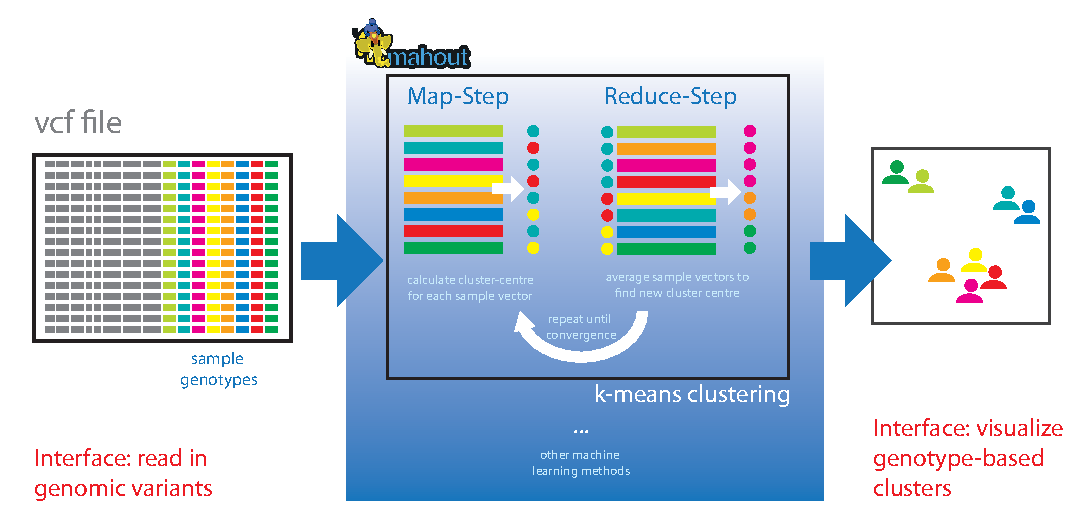
\includegraphics[type=pdf,ext=.pdf,read=.pdf, scale=0.40]{images/signature}}
        \label{fig:sign}
        \caption{{\bf Illustration of Mahout-based clustering of genotypes.}
      The image shows how the here introduced interface converts the VCF file to a mahout usable vector-based data type. Based on k-means it illustrates how the Map-step procedure groups of vectors by their nearest cluster center and the Reduce-step averages the vectors in each group to find the new value of the updated cluster center. The mahout-produced output is then converted into a visualisation.}

\end{figure}





\section*{Acknowledgement}
A.R.O was funded by the NSW Cancer Institute Big Data Big Impact schema, F.A.B by the National Health and Medical Research Council [1051757] and D.C.B by Commonwealth Scientific and Industrial Research Organisation's Transformational Capability Platform, Science and Industry Endowment Fund and Information Management and Technology Services.
The authors would like to thank Piotr Szul and Gareth Williams for their help with setting up Hadoop on the HPC system.  

\bibliographystyle{natbib}
%\bibliographystyle{achemnat}
%\bibliographystyle{plainnat}
%\bibliographystyle{abbrv}
%\bibliographystyle{bioinformatics}
\bibliography{genotypeClustering}  
\end{document}
